% !TeX program = xelatex
\documentclass[a4paper,utf8]{ctexart}
\usepackage{report}

\def\mytitle{实验报告标题}
\def\mysubtitle{实验报告副标题}
\def\name{姓名}
\def\sno{学号}
\def\institution{学院}
\def\email{xxxx@xxx.edu.cn}

\title{
    \vspace{-2cm}
    \hrule  height 2pt \relax
    \vspace{.5cm}
    {\color{DarkRed}
    \heiti{\huge \mytitle}\\
    \mysubtitle
    }
    \vspace{.5cm}
    \hrule height 1pt \relax
    }

\author{\name\\
    \sno\\
    \institution\\
    \color{DarkRed}
    \href{mailto:\email}{\fontfamily{qcr}\selectfont\email}
    }

\date{\today}


\begin{document}

\maketitle

\section{一级标题}
\subsection{二级标题}

\section{插入图片}
\begin{figure}[H]
    \centering
    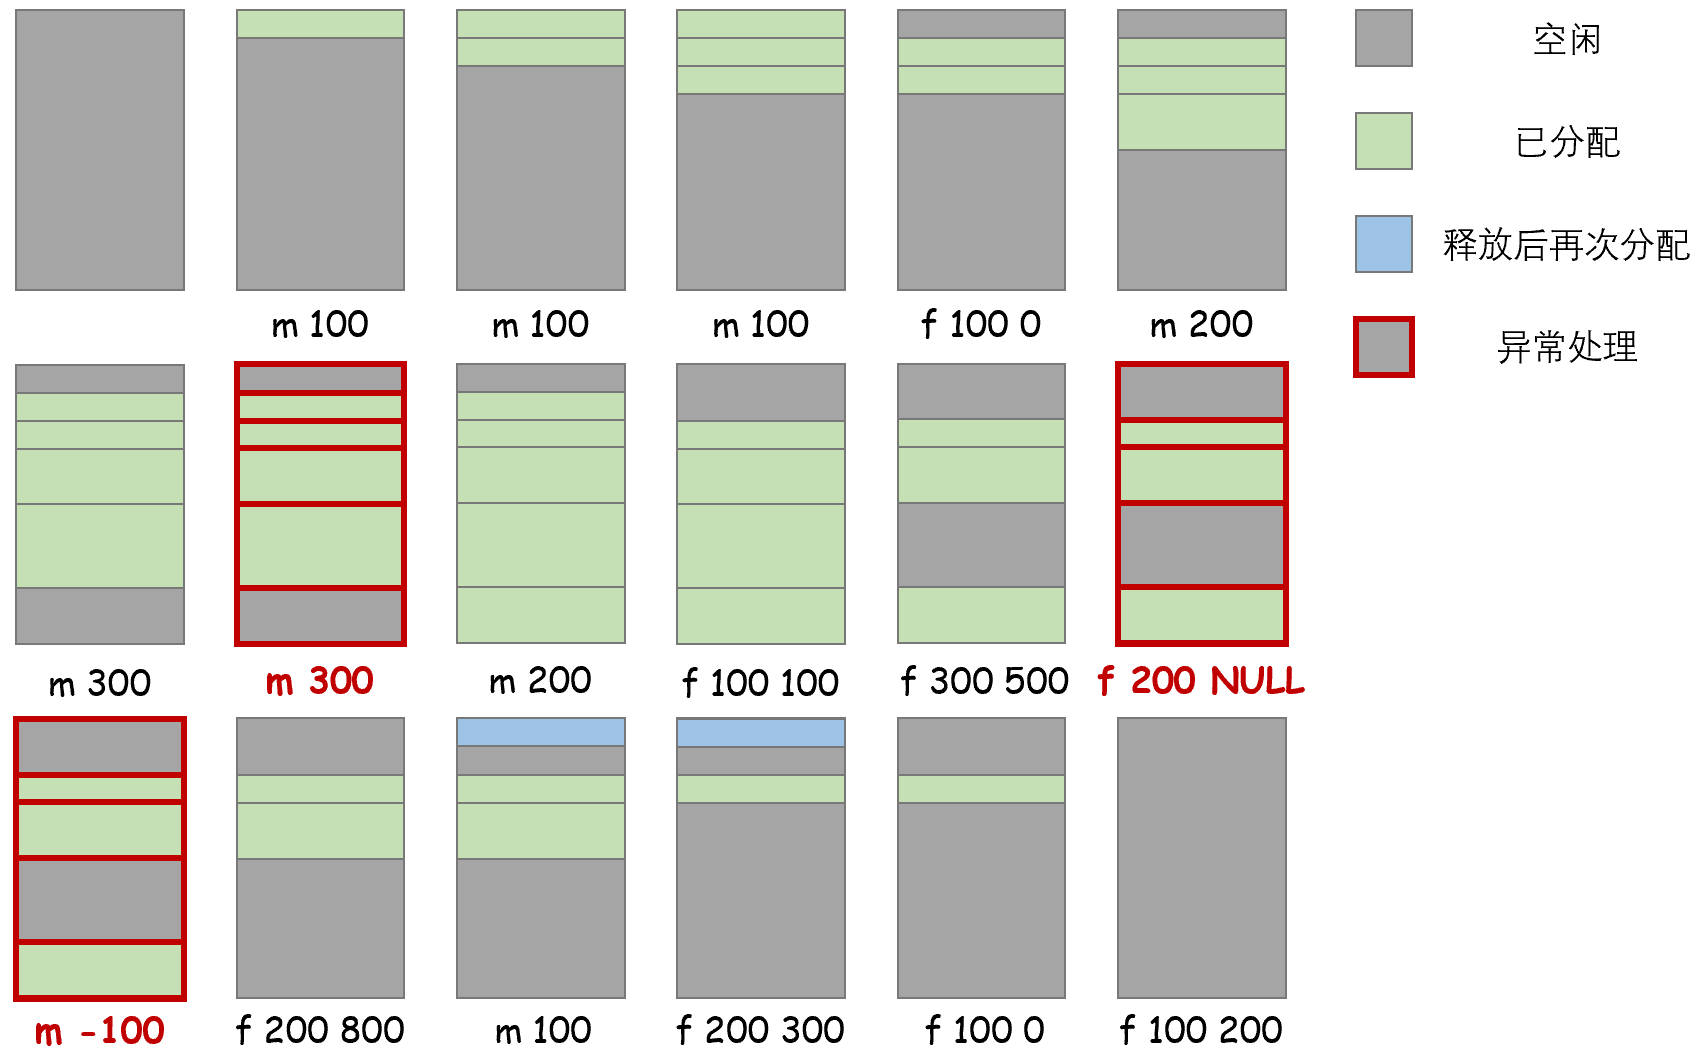
\includegraphics[width=\textwidth]{./img/example.jpg}
    \caption{测试用例示意图}
    \label{fig:example}
\end{figure}

\section{插入代码}
\begin{lstlisting}[language=C]
struct map {
    unsigned m_size;
    char *m_addr;
    struct map *next, *prior;
};
struct map *coremap;
\end{lstlisting}

% \lstinputlisting[language=C]{./code/name.c}

\appendix

\section{附录名称}

\end{document}